\begin{anexosenv}

\partanexos

\chapter{Ferramenta Shak }

\section{Uma proposta para descentralização dos serviços de internet}
Desde a sua origem, a internet foi projetada para ser uma rede
descentralizada. A grande maioria dos protocolos utilizados na rede não
dependem de pontos centrais para funcionar. De fato, é de conhecimento geral
que, por exemplo, usuários com contas de e-mails em provedores diferentes podem
trocar mensagens entre si sem qualquer problema.

O mesmo vale para outras aplicações, em especial para aquelas que utilização a
web: um blog, rede social ou site de notícias pode estar hospedado em
qualquer provedor, e não existe nenhuma razão técnica pela qual usuários que
utilizam outros provedores de acesso à rede não possam acessá-los.

Apesar disso, existe atualmente uma tendência de centralização da internet. A
imensa maioria dos usuários individuais utilizam contas de e-mail em algum
poucos grandes provedores. O mesmo acontece com utilitários como armazenamento
de documentos/arquivos/fotos, agenda, etc.

\subsection{Consequências da centralização da internet}

Essa excessiva centralização traz os seguintes problemas para a sociedade.
Entre eles, podemos citar:

\begin{description}
  \item [Riscos à privacidade]:  A quantidade de informações pessoais fornecidas 
  a serviços online
  centralizados por uma quantidade imensa de pessoas faz com que estes serviços
  representem um risco muito grande à privacidade destas pessoas. Diversos
  destes provedores mencionam explicitamente em seus termos de serviço que
  informações pessoais serão usadas para fins de marketing como exibição de
  propaganda, e não há forma de saber se são feitos outros usos dessas
  informações. Mesmo com a premissa de que os provedores de serviços são
  confiáveis, eventuais problemas de segurança em seus sistemas podem deixar
  muitas informações pessoais de muitos usuários à mercê de atacantes
  mal-intencionados (crackers, criminosos, que são popular e incorretamente
  denominados de hackers). Se essas informações estivessem dispersas em
  diversos provedores de serviços, uma eventual invasão afetaria uma quantidade
  muito menor de pessoas.

  \item [Subordinação dos usuários aos provedores]: Os grandes provedores de 
serviços acumulam uma quantidade excessiva de poder
  sobre a sociedade. Uma vez que a imensa maioria dos usuários da internet usa
  os seus serviços, estas empresas têm a capacidade de unilateralmente definir
  o que é e o que não é possível com base puramente em seus interesses
  comerciais.
  
  \item [Pontos centrais de falha]: Provedores centralizados também se tornam 
  pontos centrais de falha, e uma
  eventual indisponibilidade de seus serviços podem consequências econômicas
  gravíssimas. Na medida em que mais e mais pessoas e negócios dependem do seu
  bom andamento de suas atividades, os riscos à economia mundial se tornam cada
  vez maiores.
\end{description}

Mesmo que toda a sociedade tivesse plena consciência destes problemas causados
pela centralização dos serviços digitais, a maioria dos usuários ainda
continuaria utilizando-os, devido a um fator que acaba sendo decisivo na adoção
de provedores de serviço: a conveniência. Qualquer solução para esta questão
precisa ser no mínimo tão conveniente quanto as alternativas centralizadas
existentes na atualidade.

Este projeto visa fornecer uma alternativa à centralização da internet através
de uma solução que elimina barreira técnica para que usuários interessados
possam ter servidores próprios com aplicações sem a necessidade de conhecimento
técnico especializado. Esta solução está também norteada na maior conveniência
possível, sem sacrifício da segurança e proteção à privacidade.

\subsection{Causas da centralização da internet}

Nos últimos anos a demanda por soluções na internet vem crescendo de forma
impressionante. Por um lado, o acesso à internet aumenta mais e mais, tanto em
função do aumento da disponibilidade de conexões de banda larga, quanto a
explosão na utilização de dispositivos móveis.

Em paralelo, o tecnologia para desenvolvimento de soluções na internet avança a
passos largos, tanto no que diz respeito a possibilidades, quanto no que diz
respeito à complexidade necessária para tornar novas funcionalidades possíveis.
Serviços de alta sofisticação implicam numa alta complexidade de
desenvolvimento e manutenção.

Esta complexidade faz com que a implantação e manutenção de serviços exija
conhecimento técnico especializado. Para organizações, isto implica num maior
custo para manter sistemas e aplicações. Para indivíduos, isto quase sempre
impossibilita a manutenção de serviços próprios e leva à procura por serviços
"gratuitos". Estes serviços podem ser gratuitos do ponto de vista estritamente
financeiro e imediato, mas os termos com os quais os usuários concordam, muitas
vezes inadvertidamente, ao usar estes serviços, permitem aos provedores fazerem
uso de informações pessoais dos usuários que podem vir a ter um alto custo
tanto para o próprio indivíduo quanto para a sociedade em geral.

\subsection{Software livre como uma alternativa para a descentralização}

O conceito de Software Livre foi cunhado na década de 1980. Um Software Livre
fornece aos seus usuários 4 liberdades fundamentais:

\begin{enumerate}
  \item Executar o software para qualquer finalidade;
  \item Estudar o funcionamento do software e adaptá-lo às necessidades do usuário;
  \item Redistribuir cópias do software; 
  \item Distribuir cópias de versões modificadas do software. 
\end{enumerate}

Desde lá, o software livre se tornou parte importante da infraestrutura da
internet. Mais da metade dos servidores da internet utilizam servidores
HTTP livres. Os dos principais navegadores web (Firefox e Google Chrome) são
softwares livres, assim como é livre o sistema operacional Android, utilizado
na maioria esmagadora dos smartphones disponíveis no mercado.

Sistemas operacionais livres, como o Debian, permitem que usuários com conhecimento
técnico para tal possam hospedar os seus próprios serviços de internet,
utilizando exatamente a mesma tecnologia que é empregada nos maiores sites
profissionais.  Todo tipo de serviço pode ser hospedado com sistemas
operacionais livres, mas esta realidade ainda está longe do usuário final.

O usuários final tem a opção de ou contratar um técnico qualificado para
fazê-lo, no entanto esta é uma barreira que é muito mais difícil de transpor,
por não ser conveniente em comparação com a alternativa: simplesmente utilizar
serviços "gratuitos" de grandes players da internet, em troca de acesso às
suas informações pessoais, cedidas de forma consciente ou não, e com todas as
consequências negativas já mencionadas anteriormente.

Um outro impeditivo para que usuários possam hospedar os seus próprios serviços
de internet é o custo de manutenção do servidor em si, e de sua conectividade.
Nos últimos anos, no entanto, este fator vem perdendo relevância em função de
dois fenômenos. Por um lado, o barateamento do acesso a servidores virtuais
privados decorrente os avanços da "computação em nuvem". Por outro lado, a
disponibilidade de servidores físicos de dimensão reduzida e baixo consumo de
energia, em conjunto com o barateamento de conexões de banda larga à internet.

As inovações na computação em nuvem (especialmente em virtualização e
armazenamento) fazem com que atualmente seja possível alugar servidores
virtuais privados (VPS, da singla em inglês "virtual private server") em
provedores comerciais por valores tão baixos quanto 5 dólares por mês. Mesmo
que o valor não pareça ser tão baixo, a depender do serviço um único VPS pode
servir uma quantidade razoável de usuários, possibilitando que um grupo de
usuários possam dividir este custo.

Por outro lado, servidores virtuais em data centers comerciais também deixam
uma pula atrás da orelha dos usuários mais preocupados com a sua privacidade. A
segurança e a integridade dos dados hospedados em um VPS estão sujeitos à
confiabilidade do provedor: sendo o dono do hardware onde o VPS está
hospedado, o provedor teria em tese acesso total a tudo que está hospedado nele
mesmo num VPS individual.

Em situações onde nem um VPS oferece as garantias de privacidade necessárias,
usuários têm ainda a alternativa de hospedar os serviços em hardware próprio
em casa, utilizando a conectividade oferecida por uma conexão banda larga.
Existem hoje no mercado uma grande quantidade de servidores de dimensão
reduzida (e.g. do tamanho de um modem ADSL, ou menores), que possuem um consumo
de energia mínimo. Projetos como Freedombox apostam em servidores
físicos e privados hospedados em domicílios, em conjunto com a utilização de
criptografia, como uma saída para privacidade de fato nas comunicações
online.

\section{A Proposta}

Este projeto visa a desenvolver uma plataforma chamada shak cujo objetivo é
facilitar ao máximo que usuários sem conhecimento técnico possam ter os seus
próprios serviços de internet, garantindo sua privacidade e segurança. Esta
plataforma está concebida de acordo com os seguintes princípios:

\subsection{Base: pacotes Debian}

A plataforma shak é baseada no sistema de pacotes do Debian, uma das
distribuições GNU/Linux mais consolidadas e com maior comunidade internacional.

Os pacotes do Debian fornecem atualizações consistentes de correção e de
segurança, e são utilizados por uma grande quantidade de usuários que
reportam problemas a serem resolvidos. Porém, para garantirem uma
flexibilidade e suportar diferentes casos de uso, normalmente os pacotes não
realizam a configuração completa do ambiente, deixando os detalhes finais
para o administrador do sistema.

Além disso, normalmente aplicações são compostas de diversos pacotes, e
requerem configurações que dizem respeitos a mais de um deles e que por
consequência não poderiam ser feitas automaticamente de uma forma sustentável
em nenhum dos pacotes.

\subsection{Nova abstração: aplicação}

Para resolver as questões que não podem ser resolvidas no nível de pacotes, o
shak introduz uma nova abstração: a aplicação. Uma aplicação geralmente
contém mais de um pacote, e é responsável por toda a configuração, inclusive
configurações em múltiplos pacotes.

Concretamente, uma vez que o usuário seleciona uma determinada aplicação para
ser instalada, os pacotes necessários são instalados e as configurações
necessárias são feitas de forma automática, fornecendo de fato um "instalador
de um clique" para aplicações suportadas.

Todas as configurações são feitas de forma consistente utilizando um framework
comum, buscando o maior nível de segurança possível, e assumindo premissas que
não poderiam ser assumidas no nível da abstração pacote.

\subsection{Diferencial} para outras soluções existentes

Existem outras soluções disponíveis para "instaladores de um clique" no
mercado, mas o shak se diferencia delas nos seguintes aspectos:

\begin{enumerate}
  \item O shak pode ser implantando em um VPS na nuvem ou em servidores físicos
  próprios, a critério do usuário.
  \item O shak reutiliza o trabalho dos mantenedores Debian, que fornecem pacotes
  de alta qualidade.
  \item Por outro lado, apenas software que esteja empacotado no Debian estará
  disponível, mas isso pode ser visto de forma positiva também: o shak
  fornecerá um incentivo para que ainda mais software esteja disponível no
  Debian, o que é um benefício coletivo para o ecossistema do software livre, e
  para os seus usuários.
\end{enumerate}

O shak reutiliza a infraestrutura do projeto Debian. O Debian possui espelhos 
do seu repositório espalhados por todo o mundo, fornecendo links para 
downloads mais rápidos aonde quer que o usuário esteja. Atualizações de 
defeitos e correções de segurança realizadas no Debian estarão automaticamente 
disponíveis para usuários do shak de forma transparente. Além disso, o 
próprio shak estará disponível como um pacote dentro do próprio repositório oficial do Debian.

\chapter{Dependências do Noosfero}

\begin{longtable}[H]{l|l}
				\caption{Dependências do Noosfero nos repositórios Debian e Noosfero}\\
        \hline
        Repositório do Noosfero Debian Jessie & Repositório oficial do Debian Jessie                   \\ \hline
        bundler (1.10.6)                                 & bundler (1.7.4-1)                                                 \\ 
        Noosfero Apache (1.5)                            & inexistente                                                       \\ 
        Noosfero Chat (1.5)                              & Inexistente                                                       \\ 
        Rails (4.2.5)                                    & Rails (4.1.8-1+deb8u2)                                            \\ 
        ruby-actionmailer (4.2.5)                        & ruby-actionmailer (4.1.8)                                         \\ 
        ruby-actionpack-page-caching (1.0.2)             & Apenas na versão testing/unstable (1.2.0)  \\ 
        ruby-actionpack (4.2.5)                          & ruby-actionpack (4.1.8)                                           \\ 
        ruby-actionview (4.2.5)                          & ruby-actionview (4.1.8)                                           \\ 
         ruby-activejob (4.2.5)                          & Apenas na versão testing/unstable (4.2.6)  \\ 
        ruby-activemodel (4.2.5)                         & ruby-activemodel (4.1.8)                                          \\ 
        ruby-activerecord-deprecated-finders (1.0.4)     & ruby-activerecord-deprecated-finders (1.0.3)                      \\ 
        ruby-activerecord-session-store (0.1.1)          & Apenas na versão testing/unstable (1.0.0)  \\ 
        ruby-activerecord (4.2.4)                        & ruby-activerecord (4.1.8)                                         \\ 
        ruby-activesupport (4.2.5.1)                     & ruby-activesupport (4.1.8)                                        \\ 
        ruby-acts-as-taggable-on (3.5.0)                 & ruby-acts-as-taggable-on (2.4.1)                                  \\ 
         ruby-api-pagination (4.2.0)                     & Apenas na versão testing/unstable (4.2.0)  \\ 
        ruby-arel (6.0.3)                                & ruby-arel (5.0.1)                                                 \\ 
        ruby-axiom-types (0.1.1)                         & ruby-axiom-types (0.1.1)                                         \\ 
        ruby-binding-of-caller (0.7.2)                   & Apenas na versão testing/unstable (0.7.2)  \\ 
        ruby-byebug (5.0.0)                              & Apenas na versão testing/unstable (5.0.0)  \\ 
        ruby-chronic (0.10.2)                            & ruby-chronic (0.10.2)                                             \\ 
        ruby-coffee-rails (4.1.0)                        & ruby-coffee-rails (4.0.1)                                         \\ 
        ruby-columnize (0.9.0)                           & ruby-columnize (0.8.9)                                            \\ 
        ruby-cucumber-rails (1.4.2)                      & Apenas na versão testing/unstable (1.4.2)  \\ 
        ruby-dalli (2.7.4)                               & Apenas na versão testing/unstable (2.7.4)  \\ 
        ruby-debug-inspector (0.0.2)                     & Apenas na versão testing/unstable (0.0.2)  \\ 
         ruby-delayed-job-active-record (4.0.3)          & Apenas na versão testing/unstable (4.0.3)  \\ 
        ruby-delayed-job (4.0.6)                         & Apenas na versão testing/unstable (4.0.6)  \\ 
        ruby-doorkeeper (2.2.1)                          & Apenas na versão testing/unstable (3.1.0)  \\ 
        ruby-eita-jrails (0.10.0)                        & Inexistente no Debian                                             \\ 
        ruby-fast-gettext (0.9.2)                        & ruby-fast-gettext (0.9.0)                                         \\ 
        ruby-globalid (0.3.6)                            & Apenas na versão testing/unstable (0.3.6)  \\ 
        ruby-grape-entity (0.4.8)                        & Apenas na versão testing/unstable (0.5.1)  \\ 
        ruby-grape-logging (1.1.2)                       & Apenas na versão testing/unstable (1.3.0)  \\ 
        ruby-grape (0.12.0)                              & Apenas na versão testing/unstable (0.16.0) \\ 
        ruby-hashie (3.4.2)                              & ruby-hashie (2.0.5)                                               \\ 
        ruby-i18n (0.7.0)                                & ruby-i18n (0.6.9)                                                 \\ 
        ruby-ice-nine (0.11.1)                           & ruby-ice-nine (0.11.0)                                            \\ 
        ruby-launchy-shim (2.3.0)                        & Apenas na versão testing/unstable (2.3.0)  \\ 
        ruby-liquid (3.0.4)                              & ruby-liquid (2.6.1)                                               \\ 
        ruby-loofah (2.0.3)                              & Apenas na versão testing/unstable (2.0.3)  \\ 
        ruby-minitest-reporters (1.0.19)                 & Apenas na versão testing/unstable (1.0.19) \\ 
        ruby-molinillo (0.2.3)                           & Apenas na versão testing/unstable (0.5.0)  \\ 
        ruby-oauth2 (1.0.0)                              & ruby-oauth2 (0.9.3)                                               \\ 
        ruby-omniauth-google-oauth2 (0.2.6)              & ruby-omniauth-google-oauth2 (0.2.4)                               \\ 
        ruby-omniauth-oauth2 (1.3.1)                     & ruby-omniauth-oauth2 (1.1.2)                                      \\ 
        ruby-omniauth (1.3.1)                            & ruby-omniauth (1.2.1)                                             \\ 
        ruby-pothoven-attachment-fu (3.2.16)             & Inexistente no Debian                                             \\ 
        ruby-progressbar (1.4.2)                         & ruby-progressbar (0.21.0)                                         \\
        ruby-protected-attributes (1.1.3)                & ruby-protected-attributes (1.0.8)                                  \\
        ruby-rack-accept (0.4.5)                         & ruby-rack-accept (0.4.5)                                  \\
        ruby-rack-contrib (1.3.0)                        & Apenas na versão testing/unstable (1.3.0)                                  \\
        ruby-rack-mount (0.8.3)                          & Apenas na versão testing/unstable (0.8.3)                                  \\
        ruby-rack (1.6.4)                                & ruby-rack (1.8.3)                                  \\
        ruby-rails-deprecated-sanitizer (1.0.3)          & Apenas na versão testing/unstable (1.0.3)                                  \\
        ruby-rails-dom-testing (1.0.6)                   & Apenas na versão testing/unstable (1.0.6)                                  \\
        ruby-rails-html-sanitizer (1.0.2)                & Apenas na versão testing/unstable (1.0.3)                                  \\
        ruby-rails-observers (0.1.2)                     & ruby-rails-observers (0.1.1)                                  \\
        ruby-railties (4.2.4)                            & ruby-railties (4.2.6)                                  \\
        ruby-rakismet (1.5.2)                            & Inexistente no Debian                                  \\
        ruby-rspec-rails (3.3.3)                         & Apenas na versão testing/unstable (2.14.2)                                  \\
        ruby-selenium-webdriver (2.50.0)                 & Inexistente no Debian                                  \\
        ruby-spy (0.4.2)                                 & Apenas na versão testing/unstable (0.4.3)                                  \\
        ruby-thread-order (1.1.0)                        & Apenas na versão testing/unstable (1.1.0)                                  \\
        ruby-thread-safe (0.3.5)                         & ruby-thread-safe (0.3.1)                                  \\
        ruby-turbolinks (2.5.3)                          & ruby-turbolinks (2.2.2)                                  \\
        ruby-web-console (2.2.1)                         & Apenas na versão testing/unstable (2.2.1)                                  \\
        ruby-whenever (0.9.4)                            & Apenas na versão testing/unstable (0.9.4)                                  \\
        ruby-will-paginate (3.0.7)                       & ruby-will-paginate (3.0.5)                                  \\
        ruby-xpath (2.0.0)                               & ruby-xpath (2.0.0)                                  \\
        \hline
				\label{tabela1}
\end{longtable}

\chapter{Protótipo da interface web}
\label{prototiposhak}

O protótipo foi pensado em três áreas para o usuário, a primeira delas é na figura
\ref{fig:shakx1} e na figura \ref{fig:shakx1.2}, onde
o usuário pode ver as aplicações disponíveis, além da aplicação que possui a maior
quantidade de instalações.

\begin{figure}[h]
  \centering
  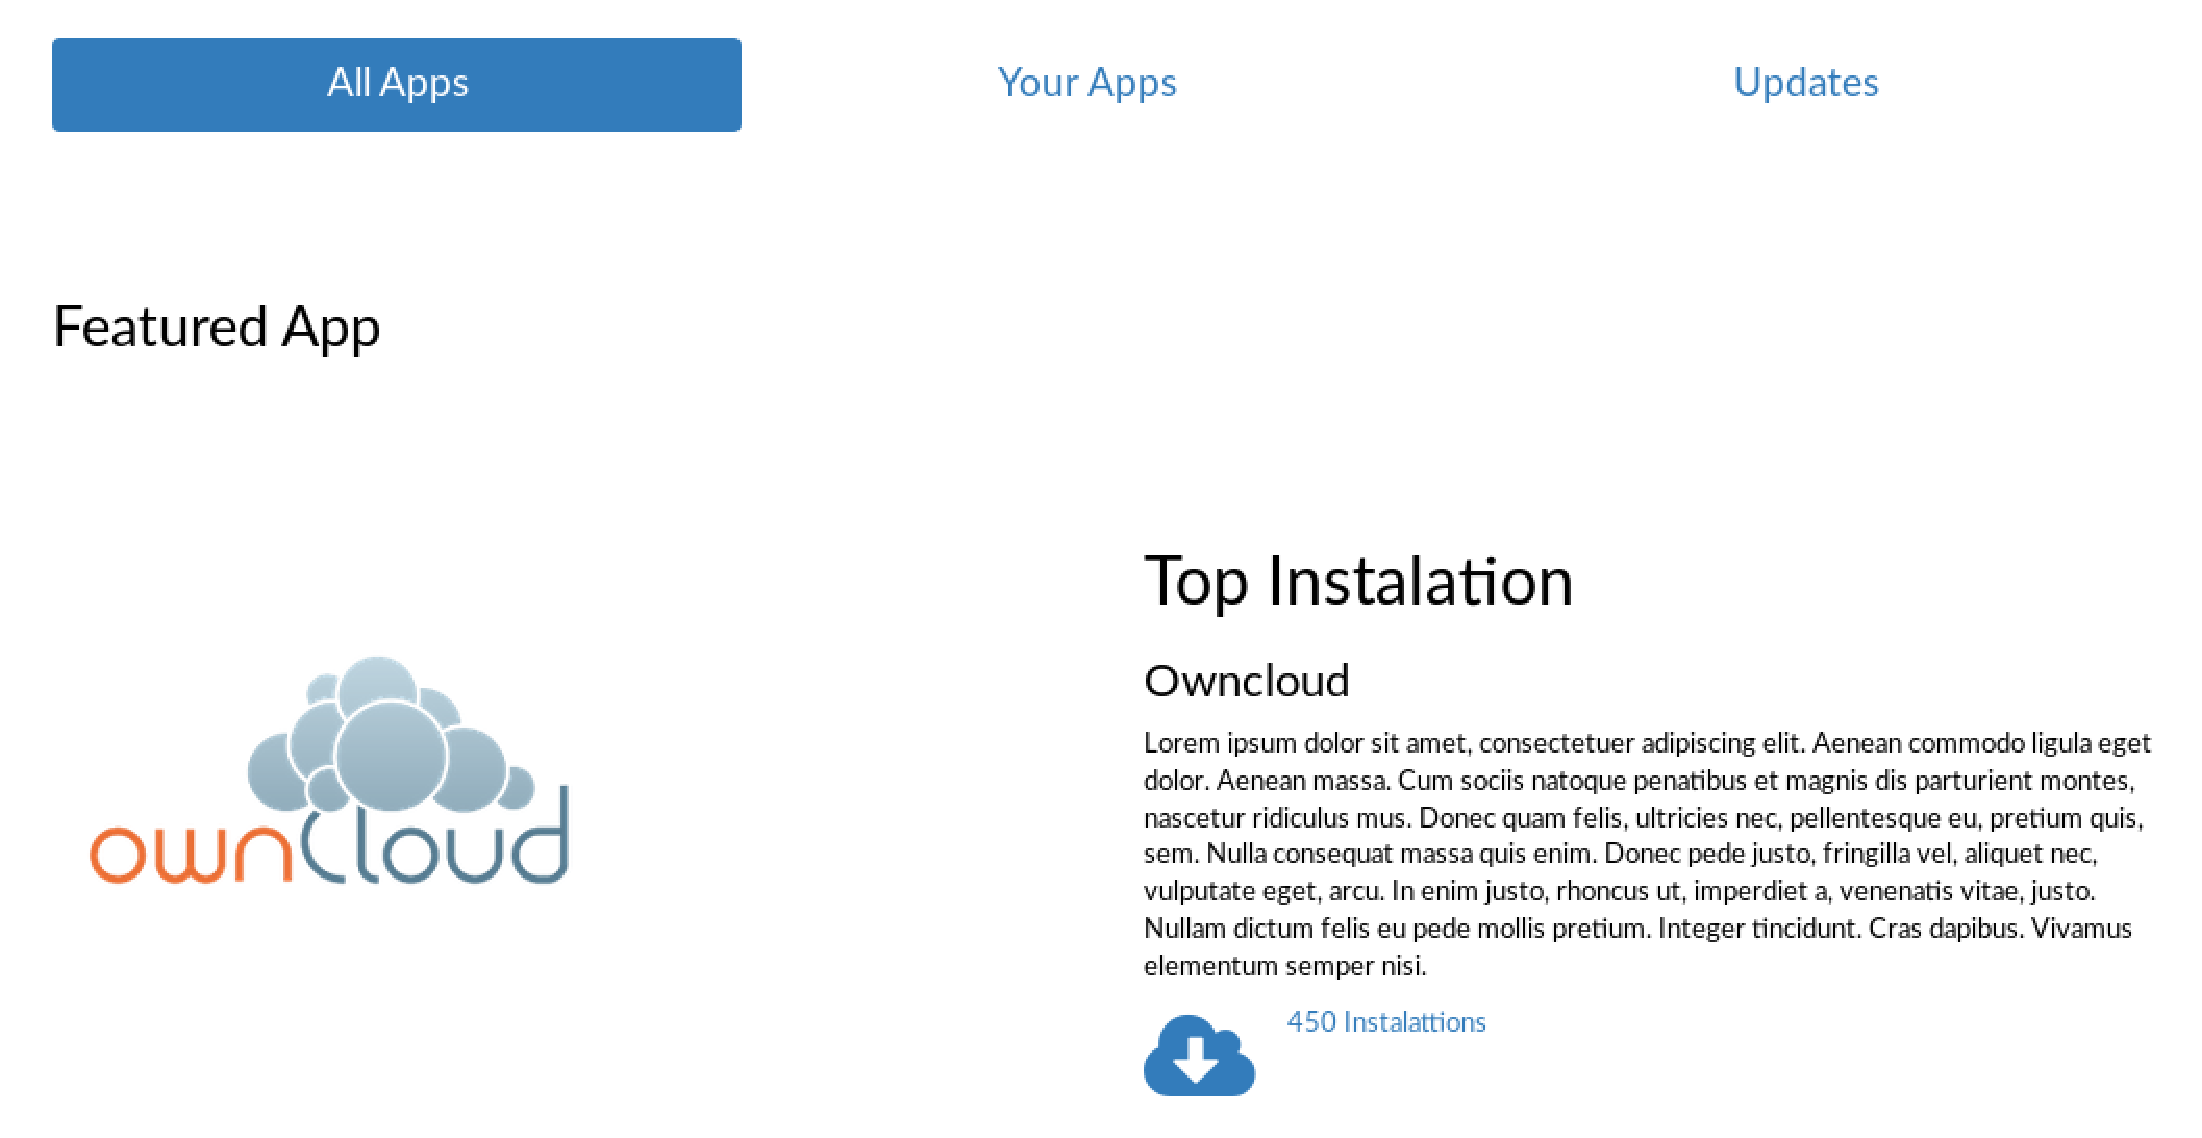
\includegraphics[width=0.8\textwidth]
      {figuras/shak1}
      \caption{Aplicação mais instalada pelo Shak}
  \label{fig:shakx1}
\end{figure}

\begin{figure}[H]
  \centering
  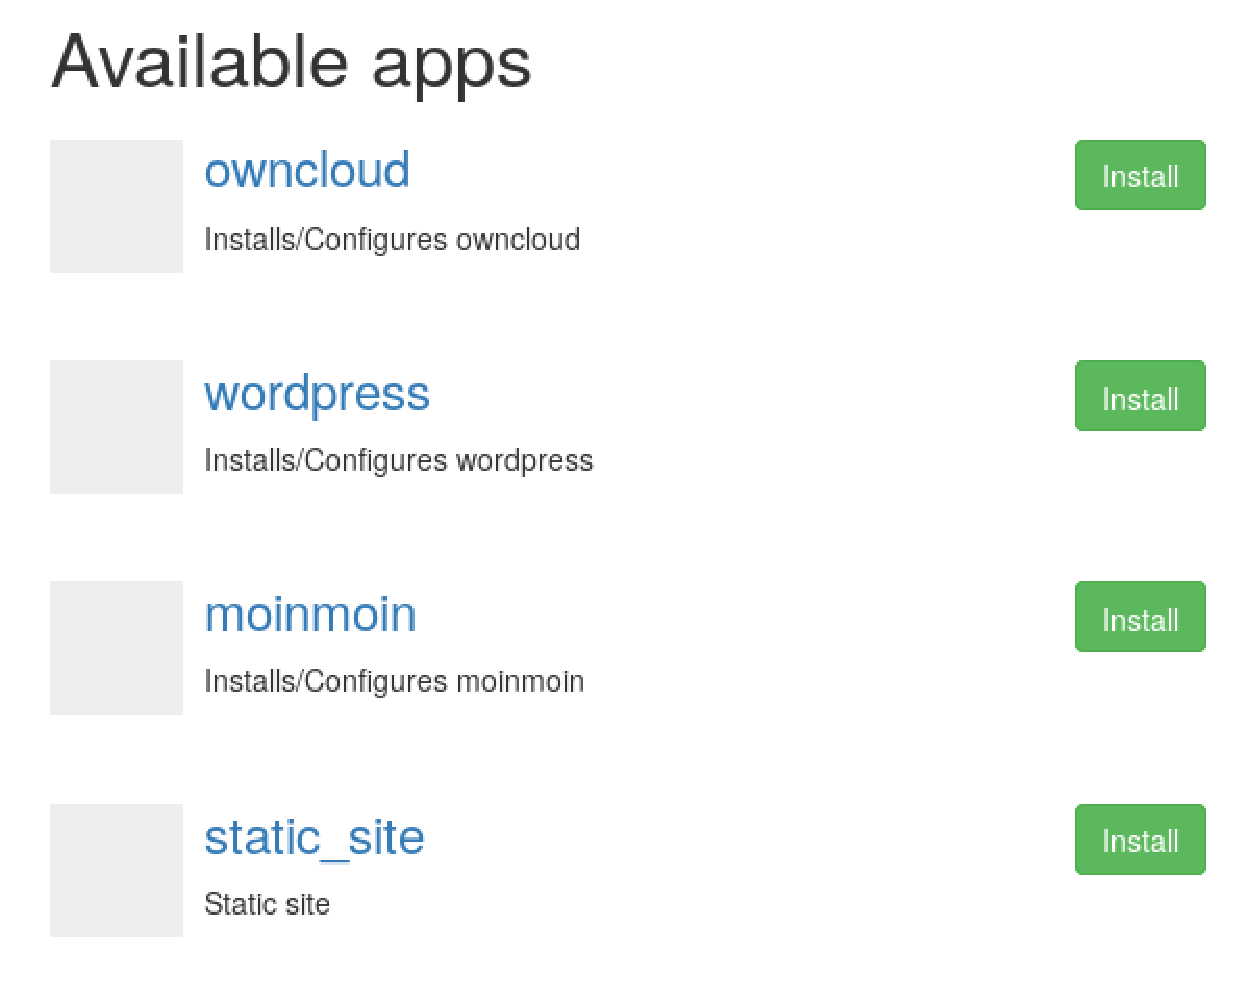
\includegraphics[width=0.8\textwidth]
      {figuras/shak1-2}
      \caption{Aplicações disponíveis para instalação}
  \label{fig:shakx1.2}
\end{figure}

Na figura \ref{fig:shakx2}, é onde o usuário pode ver suas aplicações instaladas e editar
suas informações.

\begin{figure}[H]
  \centering
  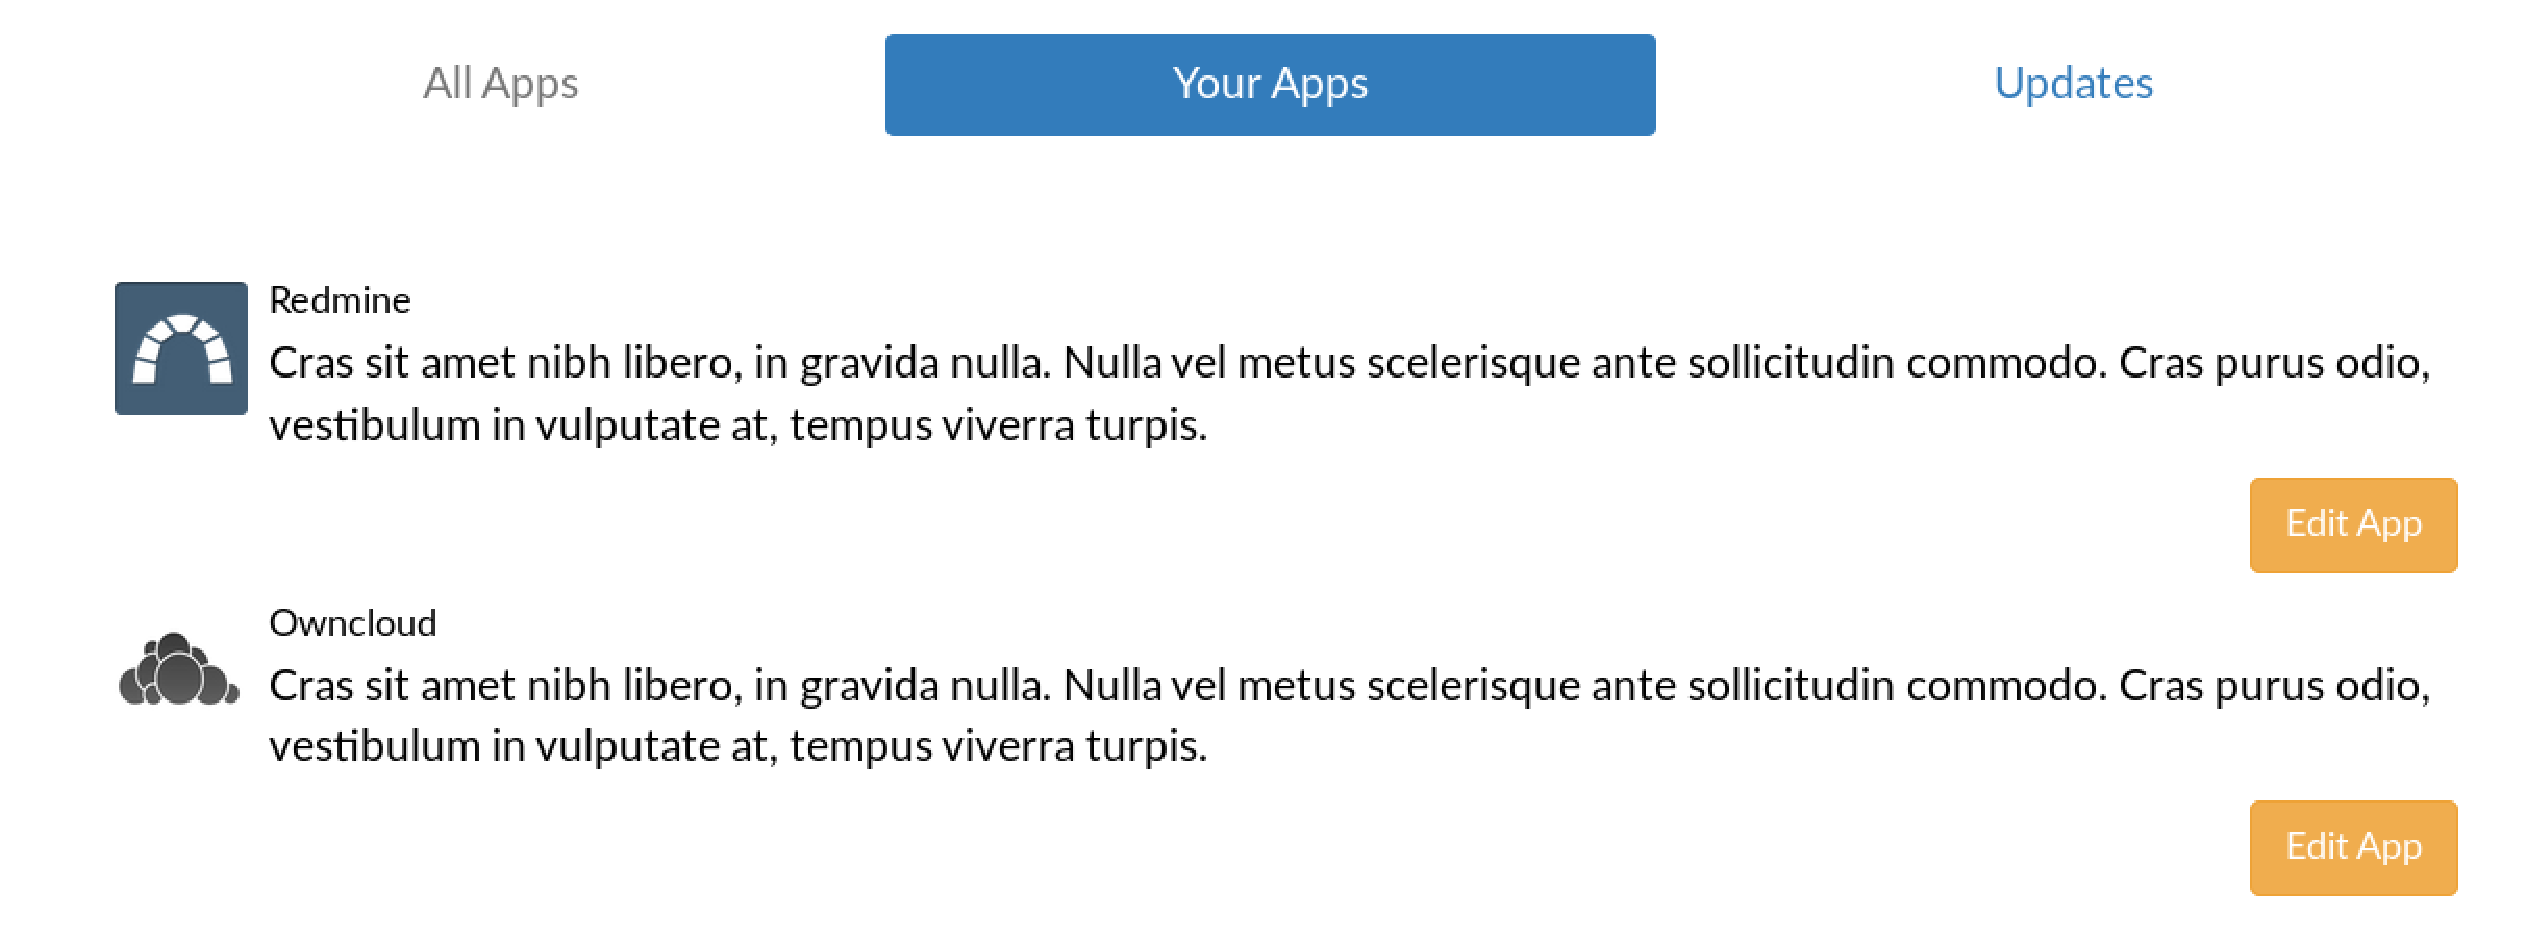
\includegraphics[width=0.8\textwidth]
      {figuras/shak2}
      \caption{Aplicações já instaladas pelo Shak}
  \label{fig:shakx2}
\end{figure}

Por fim, na figura \ref{fig:shakx3}, é onde o usuário pode atualizar suas aplicações.

\begin{figure}[H]
  \centering
  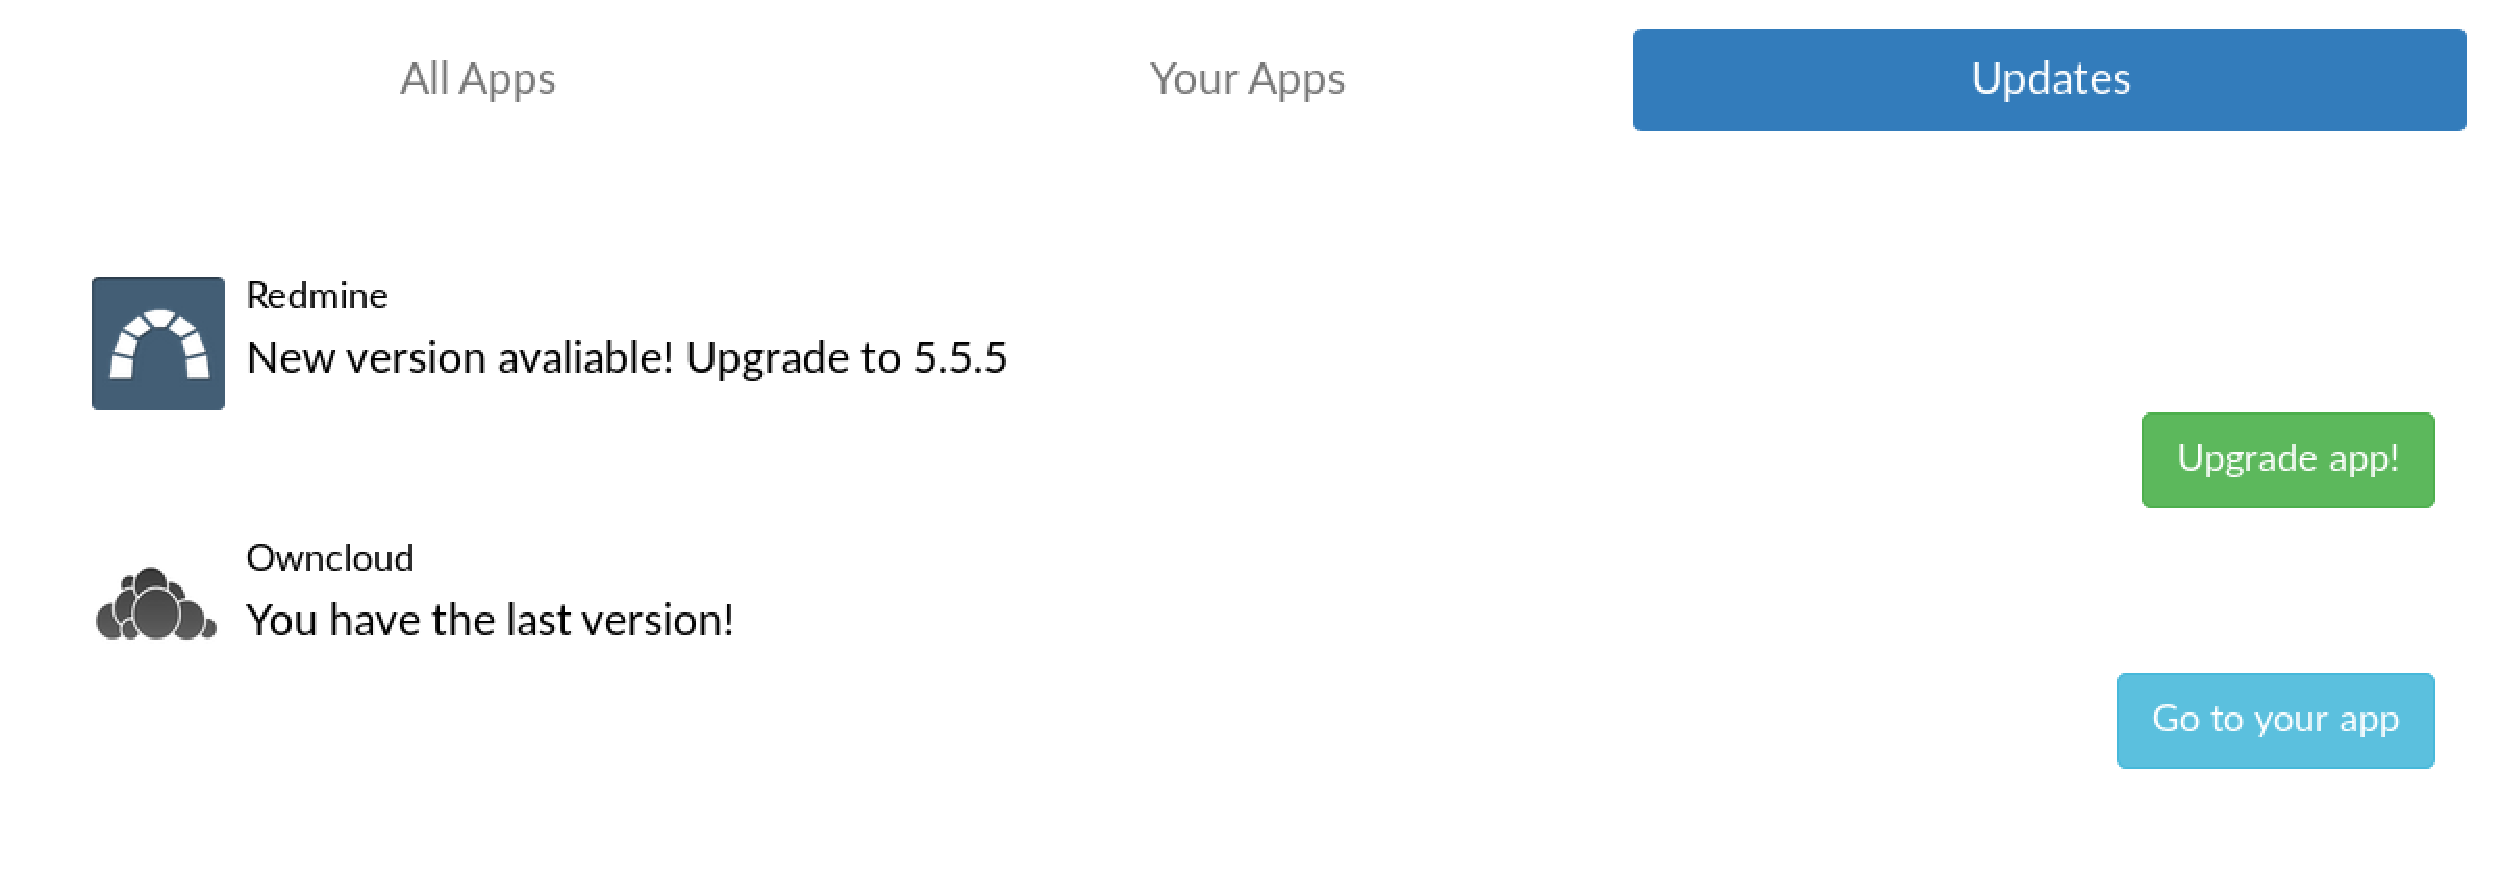
\includegraphics[width=0.8\textwidth]
      {figuras/shak3}
      \caption{Aplicações com atualizações disponíveis}
  \label{fig:shakx3}
\end{figure}

\end{anexosenv}
